\chapter{Keyboard Shortucts}
\label{shortcuts}

This chapter lists all of the keyboard shortcuts available in \texnicle. However, Mountain Lion has a useful feature that allows users to create custom shortcuts for individual applications.

To access this feature, open the \keys{Keyboard} panel in System Preferences. Navigate to \keys{Keyboard Shortcuts} and select \keys{Application Shortcuts}. Click the \keys{\ensuremath{+}} button and select \texnicle from the list.
\begin{figure}[htbp]
\centering
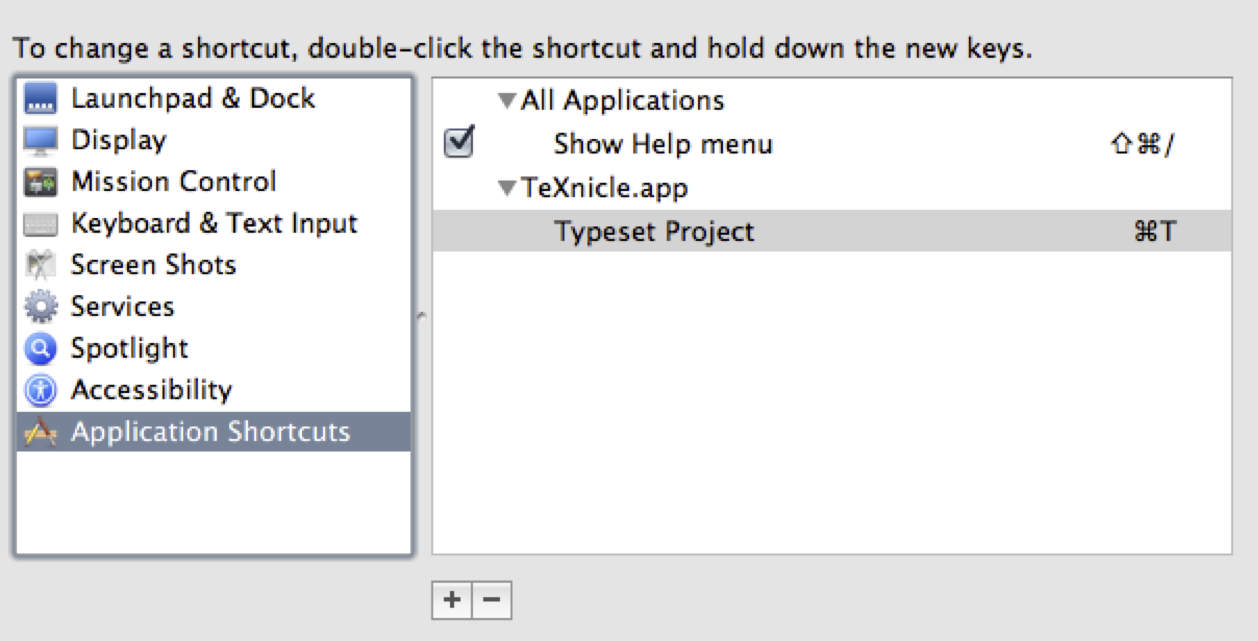
\includegraphics[width=0.5\textwidth]{TeXnicle-Images/texnicle-customshortcut.png}
\caption{Here, the Typesetting command has been remapped.}
\label{fig:texnicle-customshortcut}
\end{figure}

And now, a list of keyboard shortcuts in {\texnicle}:

\begin{description}
	\item[\keys{\cmdkey + {,}}] Open the Preferences panel.
	\item[\keys{\cmdkey + Q}] Quit \texnicle.
	\item[\keys{\cmdkey + N}] Open a new \LaTeX\ document.
	\item[\keys{\shiftkey + \cmdkey + N}] Create a new empty project.
	\item[\keys{\cmdkey + O}] Open an existing file.
	\item[\keys{\cmdkey + W}] Close the open window.
	\item[\keys{\cmdkey + S}] Save the document.
	\item[\keys{\shiftkey + \cmdkey + S}] Save the document as\ldots
	\item[\keys{\cmdkey + P}] Print.
	\item[\keys{\shiftkey + \cmdkey + P}] Page setup.
	\item[\keys{\cmdkey + Z}] Undo.	
	\item[\keys{\shiftkey + \cmdkey + Z}] Redo.
	\item[\keys{\cmdkey + X}] Cut the selected text.
	\item[\keys{\cmdkey + C}] Copy the selected text.
	\item[\keys{\cmdkey + V}] Paste the contents of the pasteboard.
	\item[\keys{\optkey + \cmdkey + V}] Paste the contents of the pasteboard as an image.
	\item[\keys{\ctlkey + \cmdkey + V}] Paste the contents of the pasteboard as a table.
	\item[\keys{\cmdkey + A}] Select all.
	\item[\keys{\ctlkey + Q}] Reformat paragraph.
	\item[\keys{\esckey}] Smart complete.
	\item[\keys{\ctlkey + Space}] Quick spell.
	\item[\keys{\cmdkey + F}] Document Find.
	\item[\keys{\shiftkey + \cmdkey + F}] Project Find.
	\item[\keys{\cmdkey + J}] Find text selection in PDF{.}
	\item[\keys{\shiftkey + \cmdkey + J}] Find PDF selection in source.
	\item[\keys{\cmdkey + G}] Find next.
	\item[\keys{\shiftkey + \cmdkey + G}] Find previous.
	\item[\keys{\cmdkey + E}] Use selection for Find.
	\item[\keys{\cmdkey + {:}}] Show spelling and grammar.
	\item[\keys{\cmdkey + {;}}] Check spelling and grammar of document now.
	\item[\keys{\optkey + \cmdkey + Space}] Open the special characters panel.
	\item[\keys{\optkey + \cmdkey + T}] Hide and show the toolbar.
	\item[\keys{\optkey + \cmdkey + F}] Enter or exit full screen.
	\item[\keys{\optkey + \cmdkey + 1}] Show Project Tree in the Navigator.
	\item[\keys{\optkey + \cmdkey + 2}] Show Symbol Palette in the Navigator.
	\item[\keys{\optkey + \cmdkey + 3}] Show Clippings Library in the Navigator.
	\item[\keys{\optkey + \cmdkey + 4}] Show Document Outline in the Navigator.
	\item[\keys{\optkey + \cmdkey + 5}] Show Project Search in the Navigator.
	\item[\keys{\optkey + \cmdkey + 6}] Show Project Information in the Navigator.
	\item[\keys{\optkey + \cmdkey + 7}] Show Project Settings in the Navigator.
	\item[\keys{\cmdkey + \ensuremath{+}}] Zoom in.
	\item[\keys{\cmdkey + \ensuremath{-}}] Zoom out.
	\item[\keys{\shiftkey + \cmdkey + N}] Create a new project.
	\item[\keys{\optkey + \cmdkey + N}] Create a new \LaTeX\ file.
	\item[\keys{\shiftkey + \cmdkey + B}] Show bookmarks.
	\item[\keys{\cmdkey + D}] Toggle bookmark for the current line.
	\item[\keys{\cmdkey + \delkey}] Delete selected bookmark.
	\item[\keys{\ctlkey + \cmdkey + B}] Jump to selected bookmark.
	\item[\keys{\ctlkey + \cmdkey + P}] Jump to previous bookmark.
	\item[\keys{\ctlkey + \cmdkey + N}] Jump to next bookmark.
	\item[\keys{\shiftkey + \cmdkey + M}] Jump to main file.
	\item[\keys{\shiftkey + \cmdkey + A}] Add existing file.
	\item[\keys{\shiftkey + \optkey + \cmdkey + A}] Add existing folder.
	\item[\keys{\shiftkey + \optkey + \cmdkey + M}] Insert in-line math mode.
	\item[\keys{\cmdkey + L}] Go to line.
	\item[\keys{\cmdkey + [}] Increase indentation.
	\item[\keys{\cmdkey + ]}] Decrease indentation.
	\item[\keys{\cmdkey + /}] Toggle comment for the current line.
	\item[\keys{\optkey + \cmdkey + /}] Increase comment level.
	\item[\keys{\ctlkey + \cmdkey + /}] Decrease comment level.
	\item[\keys{\cmdkey + \returnkey}] Jump to next placeholder.
	\item[\keys{\shiftkey + \cmdkey + \returnkey}] Jump to previous placeholder.
	\item[\keys{\cmdkey + R}] Typeset project or document.
	\item[\keys{\shiftkey + \cmdkey + R}] Typeset and view project or document in stand-alone PDF viewer.
	\item[\keys{\shiftkey + \cmdkey + K}] Trash auxiliary files.
	\item[\keys{\cmdkey + M}] Minimize window.
	\item[\keys{\optkey + \cmdkey + \tabkey}] Toggle Focus Editor/PDF{.}
	\item[\keys{\shiftkey + \cmdkey + W}] Close tab.
	\item[\keys{\shiftkey + \optkey + \cmdkey + W}] Close all tabs.
	\item[\keys{\cmdkey + \}}] Select next tab.
	\item[\keys{\cmdkey + \{}] Select previous tab.
	\item[\keys{\cmdkey +1}] Select first tab.
	\item[\keys{\cmdkey +2}] Select second tab.
	\item[\keys{\cmdkey +3}] Select third tab.
	\item[\keys{\cmdkey +4}] Select fourth tab.
	\item[\keys{\cmdkey +5}] Select fifth tab.
	\item[\keys{\optkey + \cmdkey + C}] Open the console.
	\item[\keys{\cmdkey + Q}] Quit \texnicle.\end{description}